%\section{Design Alternatives}\label{sec:alt}

\subsection{NFC Communication}\label{sec:comm}
NFC devices are typically specified for a maximum range of $10cm$. Therefore, other solutions incorporating NFC assume that the physically constrained range is enough to prevent attackers to tamper with the transmitted data.
As basic NFC hardware is quite cheap, this is probably not the right approach for the future.

A fundamental part of our \app entrance access solution is the secured NFC communication between a mobile device and a terminal installed at a gate.
This section presents building blocks ranging from low-level to high-level aspects of the NFC communication in order to achieve this goal.


\subsubsection{Hardware Setup}
Exchanging data needs a communication link between an Android smartphone and a NFC terminal.
To make it work, the NFC unit must support common NFC standards (e.g., ISO/IEC 14443) and provide stable transmission properties on the data-link layer.
Therefore, we examine our utilized hardware setup. Figure \ref{fig:nfc:hw} shows our prototype interfacing with a mobile device.
%
\begin{itemize}
	\item Raspberry Pi with a PN532 compliant NFC cape, e.g., \textit{ITEAD PN532 NFC module}.
	\item Android mobile device with NFC capabilities and Android 4.4 or newer.
\end{itemize}
%
\begin{figure}[h]
    \centering
    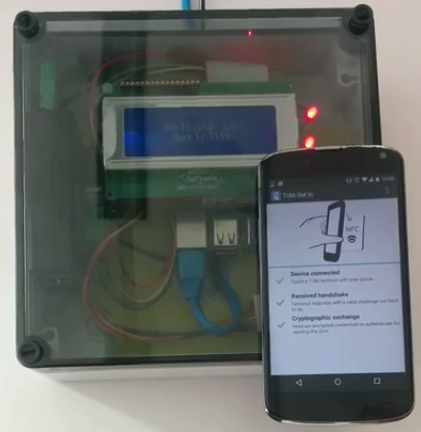
\includegraphics[width=.4\linewidth]{nfc_hardware}
    \caption{NFC hardware. Below the smartphone, there is the NFC cape that successfully finished the authentication with the smartphone.}
    \label{fig:nfc:hw}
\end{figure}
%
Using the Raspberry Pi as underlying platform and the proposed NFC transceiver, a cheap and powerful setup is possible.
It provides a rich interface to interact with the environment and allows an easy integration into existing door electronics.
For the basic operation, the free NFC library \textit{libnfc}\footnote{\url{http://nfc-tools.org/}} abstracts elementary low-level functionality like modulations for ISO/IEC 14443 standard.
It is a building block to establish a simple data-link layer for \app.

The counterpart of the terminal is a smartphone with NFC transceiver and Android 4.4 (or higher versions) that offers basic APIs to exchange data with other NFC enabled devices like our NFC cape.

\subsubsection{Low-Level Communication and Message Fragmentation}
% Card Emulation on Android side
% Terminal behaves as reader
Still, for our approach, we cannot rely on high-level APIs like Android Beam(R), for instance.
At the time of this report, it effectively only allows an one-directional communication link. The same holds for the available high-level APIs of NDEF Push.
In our case, we need a mutual authentication. This requires a bi-directional communication link.
\\
Therefore, the following architecture is used:
\begin{itemize}
	\item Android phone with Host-based Card Emulation: emulates a card based on NFC-Forum ISO-DEP specification (ISO/IEC 14443-4 in our case).
	\item NFC terminal: acts as a compliant NFC reader.
\end{itemize}
%
Given the activation, anti-collision (layer 3) and transmission properties (layer 4) are primarily managed by Android and \textit{libnfc}, an enhanced version of ISO 7816-4 layer is deployed to organize the data exchange.
It uses APDU headers to specify the type and size of data, i.e., whether the reader sends some (outgoing) chunks of data or expects the mobile device to response with some (incoming) data.

This also is the place where message fragmentation comes in.
Layer 4 can transmit messages with a maximum size of $256$ bytes.
APDU headers and status codes already consume between 2 and 5 bytes. As RSA encryption with 2048 bit alreday requires the same amount of bytes for the ciphertext, our implementation brakes down the messages into chunks with a maximum size of $125$ bytes.
According to some tests, this ensures a stable connection between the devices.
The control flow is controlled by specifying the remaining data size in the APDU status fields.

%\subsubsection{Protocols for Authentication between Smartphone and NFC Reader}\label{sec:alt:proto}
%A critical aspect in our project is the communication between a smartphone $ S $ and the NFC component $ T $.
%It is important that it is safe so that no unauthorized party can easily gain access or eavesdrop sensitive information like the student ID.
%By placing the reader's antenna in the inner side of the door, it should be safe from physical threats from outside.
%To ensure a secure communication on top of the data carrier, we plan to use one of the protocols introduced in this section.
%Which one to finally choose depends on multiple aspects like the capabilities of the NFC hardware (e.g.~processing power), Android support or fault tolerance. This needs some testing done during the project. 

\subsubsection{Protocol with Public-Key Cryptography}\label{sec:alt:proto:pubkey}
On the top level, the communication protocol relies on a local Public Key Infrastructure to establish secure communication links between the NFC participants.
For authentication on both sides and mitigation of several attack scenarios, it uses some ideas of the Needham-Schroeder-Lowe Public Key protocol. Lowe contributes an important security fix we use.
The scheme is enhanced to provide further security features specific for the utilized backend and the scenario.

%%%%%%%%%%%%%%%%%%%%%%%%%%%%%%%%%%%%%%%%%%%%%%%%%%%%%%%%%%%%%%%%%%%%%%%%%%%
% Redefine the \mess due to problems with math support $ \some_function $ %
% See: http://tex.stackexchange.com/questions/164707/how-to-use-greek-    %
%      letters-in-pgf-umlsd-or-generally-terms-starting-with              %
%%%%%%%%%%%%%%%%%%%%%%%%%%%%%%%%%%%%%%%%%%%%%%%%%%%%%%%%%%%%%%%%%%%%%%%%%%%
\renewcommand{\mess}[4][0]{
  \stepcounter{seqlevel}
  \path
  (#2)+(0,-\theseqlevel*\unitfactor-0.7*\unitfactor) node (mess from) {};
  \addtocounter{seqlevel}{#1}
  \path
  (#4)+(0,-\theseqlevel*\unitfactor-0.7*\unitfactor) node (mess to) {};
  \draw[->,>=angle 60] (mess from) -- (mess to) node[midway, above]
  {#3};
}
%
\begin{figure}[h]
	\begin{sequencediagram}
		\newinst{S}{Smartphone $ S $}
		\newinst[8.5]{T}{NFC Terminal $ T $}
		% \newinst[4]{rnc}{RNC}
		\mess{S}{1. $ {\{r_S, pseudoStudentID\}}_{K_{T-pub}} $}{T}
		\postlevel
		\mess{T}{2. $ {\{r_S, r_T\}}_{K_{S-pub}} $}{S}
		\postlevel
		\mess{S}{3. $ {\{r_T, H(salt|studentToken), commands\}}_{K_{T-pub}} $}{T}
		%\mess{nodeb}{Synchronization Indication}{rnc}
		%\filldraw[fill=black!30] ($(RRC Connection Setup to)+(0,-.3)$) rectangle ($(Synchronization Indication from) +(0,.3)$)
		%node[midway] {L1 Synchronization};
	\end{sequencediagram}
	\caption{Protocol design for secured communication between NFC terminal and mobile device.}
	\label{fig:nfc:protocol}
\end{figure}
%
\noindent
Figure \ref{fig:nfc:protocol} describes our proposed protocol.
Explanations:
%
\begin{enumerate}
	% 1.
	\item $ S \rightarrow T $:
	\begin{itemize}
		\item $ S $ generates a random number $ r_S $ and sends it to $ T $ together with the $ pseudoStudentID $, encrypted with the terminal's public key $ K_{T-pub} $. These keys are statically embedded in the Android application.
		\item The official student ID is replaced by the pseudonym $ pseudoStudentID $, which is associated with the official ID of the student in the backend.
		Like this, a MITM attack would not allow to directly gain information about the requesting person's ID.
		Furthermore, this pseudonym association can be changed regularly and at user's will.
	\end{itemize}	
	% 2.
	\item $ S \leftarrow T $:
	\begin{itemize}
		\item The terminal $ T $ looks up the public key $ K_{S-pub} $ for the pseudo student ID in the backend. If it doesn't exist, further communication stops here.
		\item On success, $ T $ generates a random number $ r_T $ and sends it back to $ S $ together with $ r_S $, encrypted with the user's public key $ K_{S-pub} $.
%		\item Providing the identity $ T $, the requesting party can verify whether the reader's public key changed. This could originate from an attack in step 1 (e.g., fake reader). In that case, abort further communication to assure confidentiality.
	\end{itemize}	
	% 3.
	\item $ S \rightarrow T $:
	\begin{itemize}
		\item If $ S $ receives a valid answer in step 2, it should be fine to proceed.
		\item $ S $ sends $ r_T $, a salted SHA-256 hash of $ studentToken $ and data to $ T $, encrypted with $ K_{T-pub} $.
		\item Having exchanged the random secrets $ r_S $ and $ r_T $ protected by the PKI, the communicating participants can be sure that these are fresh and authentic messages. Additionally, the public keys can only be fetched knowing the pseudo ID. To update a user's public key in the backend, it is necessary to sastify further conditions: secret token in addition to the real TUM student ID has to be known and the associated token must be active in TUMonline albeit a valid entry in TUM's active directory service.
		\item Salted SHA-256 student token $ H(salt|studentToken) $: as the random salt is unique per user and only known to the backend and the Android client, the terminal does not touch critical data.
		Still, by comparing the hash values received by the backend on retrieval of the user's public key, and the one sent by the smartphone in this step, the identity of the user is indirectly proven.
	\end{itemize}
\end{enumerate}